\documentclass[12pt,a4paper]{article}
\usepackage[14pt]{extsizes}
\usepackage[utf8]{inputenc}
\usepackage{amsmath}
\usepackage{amsfonts}
\usepackage{amssymb}
\usepackage{cmap}
% for fonts
    \usepackage[T2A, T1]{fontenc}
    \usepackage[english, russian]{babel}
    \usepackage{fontspec}
    \defaultfontfeatures{Ligatures=TeX,Renderer=Basic}
    \setmainfont[Ligatures={TeX, Historic}]{Times New Roman}
    \setsansfont{Times New Roman}
    \setmonofont{Courier New}
% mathcha
\usepackage{tikz}
\usepackage{mathdots}
\usepackage{yhmath}
\usepackage{cancel}
\usepackage{color}
\usepackage{siunitx}
\usepackage{array}
\usepackage{multirow}
\usepackage{amssymb}
\usepackage{gensymb}
\usepackage{tabularx}
\usepackage{booktabs}
\usetikzlibrary{fadings}
% mathcha
\usepackage{pgfplots} % plot
\usepackage{float} % for H at figure
\usepackage{cases}
\pgfplotsset{compat=1.15}
\usepackage{graphicx}
\usepackage[left=2cm,right=2cm,top=2cm,bottom=2cm]{geometry}
\author{Аверьянов Тимофей}
\begin{document}
\begin{center}
\textbf{Аверьянов Тимофей ПМ 3-1}

\textbf{Отчёт по домашней работе}
\end{center}
$\displaystyle \boxed{\text{ДЗ}}$ В качестве домашнего задания прошу проанализировать конфликты интересов двух крупных компаний в отрасли (на выбор), сформулировать стратегии конкурентного взаимодействия (не менее 3-х), задать шкалу выигрышей и построить биматричную игру.

Решить игру методом сведения к задаче \textit{смешанно-целочисленного программирования}.

\textbf{Решение:}

В качестве конфликтующих компаний была выбраны компании \textcolor[rgb]{0.29,0.56,0.89}{Яндекс} и \textcolor[rgb]{0.82,0.01,0.11}{Google}.

Пусть компании \textcolor[rgb]{0.29,0.56,0.89}{Яндекс} обозначим её игрком \textcolor[rgb]{0.29,0.56,0.89}{А} имеет следующие стратегии:

\textcolor[rgb]{0.29,0.56,0.89}{A1} - подать в суд на компанию \textcolor[rgb]{0.82,0.01,0.11}{Google} за отсутсвие предустановки приложений \textcolor[rgb]{0.29,0.56,0.89}{«Яндекса»}.

\textcolor[rgb]{0.29,0.56,0.89}{А2} - обратиться в Еврокомиссию с просьбой расследовать монополию в Android в суд на компанию \textcolor[rgb]{0.82,0.01,0.11}{Google}.

\textcolor[rgb]{0.29,0.56,0.89}{А3} - поддержать антимонопольный иск Microsoft и Nokia к \textcolor[rgb]{0.82,0.01,0.11}{Google}.

\textcolor[rgb]{0.29,0.56,0.89}{А4} - не предъявлять никаких претензий в сторону компании \textcolor[rgb]{0.82,0.01,0.11}{Google}.

У компании \textcolor[rgb]{0.82,0.01,0.11}{Google}, обозначим игроком \textcolor[rgb]{0.82,0.01,0.11}{B}, есть следующие стратегии:

\textcolor[rgb]{0.82,0.01,0.11}{B1} - подать иск в Арбитражный суд Москвы с требованием признать незаконными притензии компании \textcolor[rgb]{0.29,0.56,0.89}{Яндекс} и иски Microsoft и Nokia к \textcolor[rgb]{0.82,0.01,0.11}{Google}.

\textcolor[rgb]{0.82,0.01,0.11}{B2} - отказать Еврокомиссии в расследовании.

\textcolor[rgb]{0.82,0.01,0.11}{B3} - позволить Еврокомиссии провести расследование.

\textcolor[rgb]{0.82,0.01,0.11}{B4} - продолжать свою деятельность не предпринимая никаких действий по защите от обвинений.

Введём следующую шкалу оценивания:
\begin{table}[H]
  \begin{center}
    \begin{tabular}{|c|c|}
    \hline
     Выйгрыш компании & Описание выигрыша \\
    \hline
     0 & Компания проигрывает событие \\
    \hline
     1 & Компания скорее проигрывает событие, чем выигрывает \\
    \hline
     2 & Компания скорее выигравает событие, чем проигрывает \\
    \hline
     3 & Компания выигрывает событие \\
     \hline
    \end{tabular}
  \end{center}
\end{table}
Платежи игроков представленны матрицей $\displaystyle (( a_{ij} ,b_{ij}))$, где $\displaystyle m\ =\ n\ =4$:
\begin{equation*}
\begin{pmatrix}
( 1,3) & ( 1,2) & ( 0,1) & ( 3,1)\\
( 3,2) & ( 2,3) & ( 2,0) & ( 0,1)\\
( 2,3) & ( 1,0) & ( 1,2) & ( 3,1)\\
( 1,0) & ( 3,2) & ( 0,2) & ( 2,3)
\end{pmatrix}
\end{equation*}
Для решения данной биматричной игры необходимо составить следующие ограничения:
\begin{equation*}
\text{Ограничения \\ для игрока А}\begin{cases}
p_{i} \ < \ x_{i} & i\ =\ 1,\ \dotsc ,\ m\\
0\ \leq v_{1} \ -\ {\displaystyle \sum ^{n}_{j=1} a_{ij} q_{j} \leq U_{1}( 1-x_{i})} & i\ =\ 1,\ \dotsc ,\ m
\end{cases}
\end{equation*}
\begin{equation*}
\text{Ограничения \\ для игрока B}\begin{cases}
q_{j} \ < \ y_{j} & j\ =\ 1,\ \dotsc ,\ n\\
0\ \leq v_{2} \ -\ {\displaystyle \sum ^{m}_{i=1} a_{ij} p_{i} \leq U_{2}( 1-y_{j})} & j\ =\ 1,\ \dotsc ,\ n
\end{cases}
\end{equation*}
\begin{equation*}
\text{Дополнительные \\ ограничения}\begin{cases}
{\displaystyle \sum ^{m}_{i=1} p_{i} =1,\ \sum ^{n}_{i=1} q_{j} =1} & \\
p_{i} \ \geq 0,\ x_{i} \in \{0,1\} & i\ =\ 1,\ \dotsc ,\ m\\
q_{j} \ \geq 0,\ y_{j} \in \{0,1\} & j\ =\ 1,\ \dotsc ,\ n
\end{cases}
\end{equation*}

\begin{figure}[H]
\begin{center}
  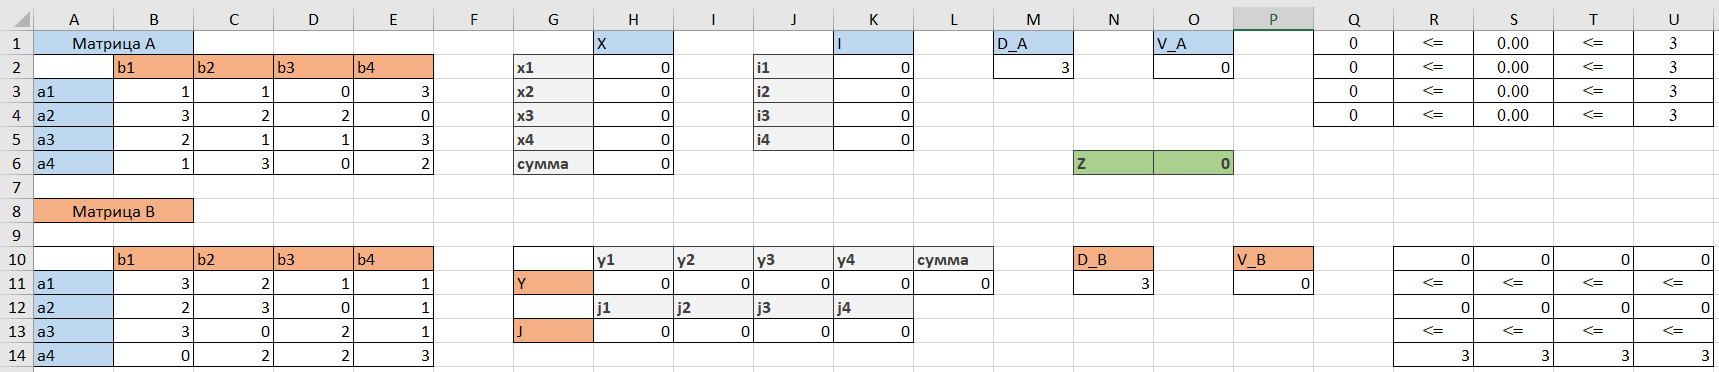
\includegraphics[width=0.9\textwidth]{img/start.PNG}
\end{center}
\end{figure}



После чего с помощью смешанно-целочиленного программирования решим эту систему с помощью функции подбора решений Excel со следующими параметрами:

\begin{figure}[H]
\begin{center}
  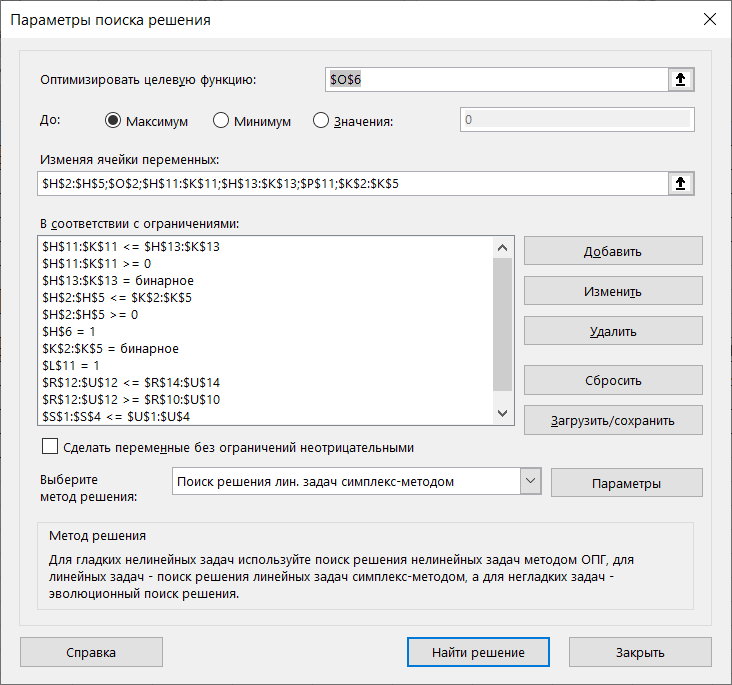
\includegraphics[width=0.9\textwidth]{img/par_solve.png}
\end{center}
\end{figure}


Указываем целевую функции ставим параметр 'Максимум', выставляем значения переменных и составляем ограния по формулам описанным выше, выставим поиск решений симплекс-методом и после всех этих действий получим следующее решение:

\begin{figure}[H]
\begin{center}
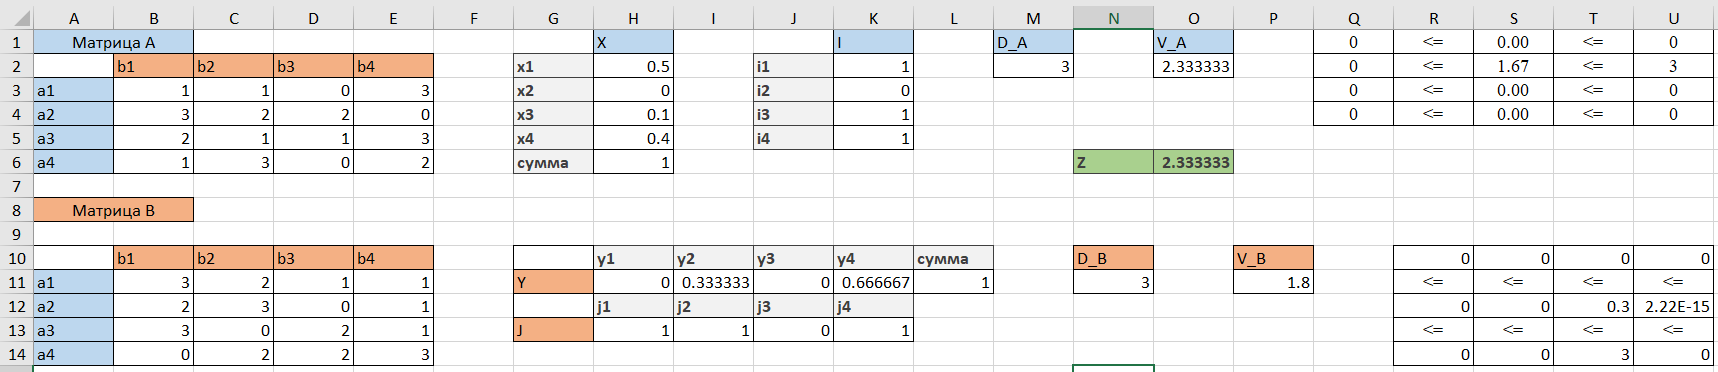
\includegraphics[width=0.9\textwidth]{img/end.PNG}
\end{center}
\end{figure}

Таким образом решение данной системы:
\begin{equation*}
p^{*} =( 0.5,0,0.1,0.4) ,q^{*} =( 0,\ 0.33,\ 0,\ 0.67) ,v^{*} =2.33
\end{equation*}
\textbf{Вывод: }Таким образом, компания Яндекс должна бросить 50\% усилий на подачу в суд на компанию Google за отсутсвие предустановки приложений «Яндекса», 10\% на поддержку антимонопольного иска Microsoft и Nokia к Google и на 40\% не предъявлять никаких претензий в сторону компании Google. Компания Google на 33\% должна отказать Еврокомиссии в расследовании и на 67\% продолжать свою деятельность не предпринимая никаких действий по защите от обвинений.
\end{document}
